\documentclass[11pt,openany]{article}

\usepackage{mathtools, commath}
% Packages for formatting
\usepackage[margin=1in]{geometry}
\usepackage{fancyhdr}
\usepackage{enumerate}
\usepackage{graphicx}
\usepackage{kotex}
\usepackage{arydshln} % Include this package
\usepackage{bbding}
\usepackage{amsmath}
\usepackage{amsthm}
\usepackage[dvipsnames,table]{xcolor}
\usepackage{amssymb, amsfonts}
\usepackage{wasysym}
\usepackage{footnote}
\usepackage{tablefootnote}
\usepackage{arydshln} % Include this package
% Fonts
\usepackage[T1]{fontenc}
\usepackage[utf8]{inputenc}
\usepackage{newpxtext,newpxmath}
\usepackage{sectsty}

% Define colors
\definecolor{TealBlue1}{HTML}{0077c2}
\definecolor{TealBlue2}{HTML}{00a5e6}
\definecolor{TealBlue3}{HTML}{b3e0ff}
\definecolor{TealBlue4}{HTML}{00293c}
\definecolor{TealBlue5}{HTML}{e6f7ff}

\definecolor{thmcolor}{RGB}{231, 76, 60}
\definecolor{defcolor}{RGB}{52, 152, 219}
\definecolor{lemcolor}{RGB}{155, 89, 182}
\definecolor{corcolor}{RGB}{46, 204, 113}
\definecolor{procolor}{RGB}{241, 196, 15}

\usepackage{color,soul}
\usepackage{soul}
\newcommand{\mathcolorbox}[2]{\colorbox{#1}{$\displaystyle #2$}}
\usepackage{cancel}
\newcommand\crossout[3][black]{\renewcommand\CancelColor{\color{#1}}\cancelto{#2}{#3}}
\newcommand\ncrossout[2][black]{\renewcommand\CancelColor{\color{#1}}\cancel{#2}}

\usepackage{hyperref}
\usepackage{booktabs}

% Chapter formatting
\definecolor{titleTealBlue}{RGB}{0,53,128}
\usepackage{titlesec}
\titleformat{\section}
{\normalfont\sffamily\Large\bfseries\color{titleTealBlue!100!gray}}{\thesection}{1em}{}
\titleformat{\subsection}
{\normalfont\sffamily\large\bfseries\color{titleTealBlue!50!gray}}{\thesubsection}{1em}{}

%Tcolorbox
\usepackage[most]{tcolorbox}
\usepackage{multirow}
\usepackage{multicol}

\usepackage[linesnumbered,ruled]{algorithm2e}
\usepackage{algpseudocode}
\usepackage{setspace}
\SetKwComment{Comment}{/* }{ */}
\SetKwProg{Fn}{Function}{:}{end}
\SetKw{End}{end}
\SetKw{DownTo}{downto}

% Define a new environment for algorithms without line numbers
\newenvironment{algorithm2}[1][]{
	% Save the current state of the algorithm counter
	\newcounter{tempCounter}
	\setcounter{tempCounter}{\value{algocf}}
	% redefine the algorithm numbering (remove prefix)
	\renewcommand{\thealgocf}{}
	\begin{algorithm}
	}{
	\end{algorithm}
	% Restore the algorithm counter state
	\setcounter{algocf}{\value{tempCounter}}
}

\usepackage{adjustbox}
% Header and footer formatting
\pagestyle{fancy}
\fancyhead{}
\fancyhf{}
\rhead{\textcolor{TealBlue2}{\large\textbf{기대수(기초부터 대학원 수학까지 시리즈) 3기}}}%\rule{3cm}{0.4pt}}
\lhead{\textcolor{TealBlue2}{\large\textbf{수학의 즐거움, Enjoying Math}}}
% Define footer
%\newcommand{\footer}[1]{
%\begin{flushright}
%	\vspace{2em}
%	\includegraphics[width=2.5cm]{school_logo.jpg} \\
%	\vspace{1em}
%	\textcolor{TealBlue2}{\small\textbf{#1}}
%\end{flushright}
%}
%\rfoot{\large Department of Information Security, Cryptogrphy and Mathematics, Kookmin Uni.\includegraphics[height=1.5cm]{school_logo.jpg}}
\fancyfoot{}
\fancyfoot[C]{-\thepage-}

\usepackage{tcolorbox}
\tcbset{colback=white, arc=5pt}

\definecolor{axiomcolor}{HTML}{a88bfa}
\definecolor{defcolor}{RGB}{52, 152, 219}
\definecolor{procolor}{RGB}{241, 196, 15}
\definecolor{thmcolor}{RGB}{231, 76, 60}
\definecolor{lemcolor}{RGB}{155, 89, 182}
\definecolor{corcolor}{RGB}{46, 204, 113}
\definecolor{execolor}{RGB}{90, 128, 127}

% Define a new command for the custom tcolorbox
\newcommand{\axiombox}[2][]{%
	\begin{tcolorbox}[colframe=axiomcolor, title={\color{white}\bfseries #1}]
		#2
	\end{tcolorbox}
}

\newcommand{\defbox}[2][]{%
	\begin{tcolorbox}[colframe=defcolor, title={\color{white}\bfseries #1}]
		#2
	\end{tcolorbox}
}

\newcommand{\lembox}[2][]{%
	\begin{tcolorbox}[colframe=lemcolor, title={\color{white}\bfseries #1}]
		#2
	\end{tcolorbox}
}

\newcommand{\probox}[2][]{%
	\begin{tcolorbox}[colframe=procolor, title={\color{white}\bfseries #1}]
		#2
	\end{tcolorbox}
}

\newcommand{\thmbox}[2][]{%
	\begin{tcolorbox}[colframe=thmcolor, title={\color{white}\bfseries #1}]
		#2
	\end{tcolorbox}
}

\newcommand{\corbox}[2][]{%
	\begin{tcolorbox}[colframe=corcolor, title={\color{white}\bfseries #1}]
		#2
	\end{tcolorbox}
}



\usepackage{amsthm}

% Define custom theorem styles
\newtheoremstyle{dotless} % Name of the style
{3pt} % Space above
{3pt} % Space below
{\itshape} % Body font
{} % Indent amount
{\bfseries} % Theorem head font
{} % Punctuation after theorem head
{2.5mm} % Space after theorem head
{} % Theorem head spec

\newtheoremstyle{definitionstyle} % Name of the style
{3pt} % Space above
{3pt} % Space below
{} % Body font
{} % Indent amount
{\bfseries} % Theorem head font
{.} % Punctuation after theorem head
{2.5mm} % Space after theorem head
{} % Theorem head spec

% Applying custom styles
\theoremstyle{dotless}
\newtheorem{theorem}{Theorem} % Theorem environment with section-wise numbering
\newtheorem{proposition}[theorem]{Proposition} % Theorem environment with section-wise numbering
\newtheorem{lemma}[theorem]{Lemma} % Lemma shares the counter with theorem
\newtheorem{corollary}[theorem]{Corollary} % Corollary shares the counter with theorem

\theoremstyle{definitionstyle}
\newtheorem*{observation}{\textcolor{Magenta}{Observation}}
\newtheorem{definition}{Definition} % Definition shares the counter with theorem
\newtheorem{example}{Example} % Example shares the counter with theorem
\newtheorem{exercise}{Exercise} % Example shares the counter with theorem
\newtheorem{remark}{Remark} % Remark shares the counter with theorem
\newtheorem*{note}{Note}

\newtheorem*{definition*}{Definition} % Definition shares the counter with theorem
\newtheorem*{example*}{Example} % Example shares the counter with theorem
\newtheorem*{exercise*}{\textcolor{violet}{Exercise}} % Example shares the counter with theorem
\newtheorem*{remark*}{Remark} % Remark shares the counter with theorem


\usepackage{tikz}
\usepackage{tikz-cd}
\usepackage{tikz-3dplot}
\usepackage{pgfplots}
\pgfplotsset{compat=newest} % Adjust to your version of pgfplots
\def\Circlearrowleft{\ensuremath{%
		\rotatebox[origin=c]{180}{$\circlearrowleft$}}}
\def\Circlearrowright{\ensuremath{%
		\rotatebox[origin=c]{180}{$\circlearrowright$}}}
\def\CircleArrowleft{\ensuremath{%
		\reflectbox{\rotatebox[origin=c]{180}{$\circlearrowleft$}}}}
\def\CircleArrowright{\ensuremath{%
		\reflectbox{\rotatebox[origin=c]{180}{$\circlearrowright$}}}}
\usetikzlibrary{
	3d, % For 3D drawing
	angles,
	arrows,
	arrows.meta,
	backgrounds,
	bending,
	calc,
	decorations.pathmorphing,
	decorations.pathreplacing,
	decorations.markings,
	fit,
	matrix,
	patterns,
	patterns.meta,
	positioning,
	quotes,
	shadows,
	shapes,
	shapes.geometric,
	tikzmark
}
\tikzset{
	% single mid‐path arrow
	mid arrow/.style={
		decoration={
			markings,
			mark=at position 0.5 with {\arrow{Stealth[scale=1.2]}}
		},
		postaction={decorate},
	},
	% style for field arrows
	field arrow/.style={
		-{Stealth[scale=1.0]},
		thick,
		blue!70!black,
	},
}
\newcommand{\ie}{\textnormal{i.e.}}
\newcommand{\rsa}{\mathsf{RSA}}
\newcommand{\rsacrt}{\mathsf{RSA}\textendash\mathsf{CRT}}
\newcommand{\inv}[1]{#1^{-1}}

%New Command
%\newcommand{\set}[1]{\left\{#1\right\}}
\newcommand{\N}{\mathbb{N}}
\newcommand{\Z}{\mathbb{Z}}
\newcommand{\Q}{\mathbb{Q}}
\newcommand{\R}{\mathbb{R}}
\newcommand{\cR}{\mathcal{R}}
\newcommand{\C}{\mathbb{C}}
\newcommand{\F}{\mathbb{F}}
\newcommand{\nbhd}{\mathcal{N}}
\newcommand{\Log}{\operatorname{Log}}
\newcommand{\Arg}{\operatorname{Arg}}
\newcommand{\pv}{\operatorname{P.V.}}

\newcommand{\of}[1]{\left( #1 \right)} 
%\newcommand{\abs}[1]{\left\lvert #1 \right\rvert}
%\newcommand{\norm}[1]{\left\| #1 \right\|}

\newcommand{\sol}{\textcolor{magenta}{\bf Sol}}
\newcommand{\conjugate}[1]{\overline{#1}}

\newcommand{\res}{\operatorname{res}}
\DeclareMathOperator*{\Res}{\operatorname{Res}}

%\renewcommand{\Re}{\operatorname{Re}}
%\renewcommand{\Im}{\operatorname{Im}}

\newcommand{\cyclic}[1]{\langle #1 \rangle}
\newcommand{\uniform}{\overset{\$}{\leftarrow}}
\newcommand{\xmark}{\textcolor{red}{\XSolidBrush}}
\newcommand{\vmark}{\textcolor{green!75!black}{\CheckmarkBold}}

\newcommand{\gen}[1]{\langle #1 \rangle}
\newcommand{\Gen}[1]{\left\langle #1 \right\rangle}

\newcommand{\img}[1]{\text{Img}(#1)}
\newcommand{\Img}[1]{\text{Img}\left(#1\right)}
\newcommand{\preimg}[1]{\text{Img}^{-1}(#1)}
\newcommand{\Preimg}[1]{\text{Img}^{-1}\left(#1\right)}

\newcommand{\relation}{\mathrel{\mathcal{R}}}
\newcommand{\injection}{\rightarrowtail}
\newcommand{\surjection}{\twoheadrightarrow}
\newcommand{\id}{\textnormal{id}}

\newcommand{\eqclass}[1]{\left[#1\right]}

% Define custom colors for O and X
\newcommand{\yes}{\textcolor{blue}{\bf \fullmoon}}
\newcommand{\no}{\textcolor{red}{\bf \texttimes}}

\DeclarePairedDelimiter\ceil{\lceil}{\rceil}
\DeclarePairedDelimiter\floor{\lfloor}{\rfloor}
%\renewcommand{\floor}[#1]{\lfloor #1\rfloor}
%\newcommand{\Floor}[#1]{\left\lfloor #1\right\rfloor}
%\newcommand{\ceil}[#1]{\lceil #1\rceil}
%\newcommand{\Ceil}[#1]{\left\lceil #1\right\rceil}

\newcommand{\topology}{\mathscr{T}}
\newcommand{\sequence}[1]{\langle #1\rangle}

\setstretch{1.25}
\begin{document}
\pagenumbering{arabic}
\begin{center}
	\huge\textbf{Algebraic Structures}\\
	\vspace{0.5em}
	\large{Ji, Yong-hyeon}\\
%	\large{\ttfamily \url{https://github.com/Hacker-Code-J}}\\
	\vspace{0.5em}
	\normalsize{\today}\\
\end{center}

\noindent 
We cover the following topics in this note.
\begin{itemize}
	\item Group, Ring, Field
	\item Vector Space, Module
\end{itemize}
\hrule\vspace{12pt}
%\tableofcontents
%\newpage

\begin{figure}[h!]\centering
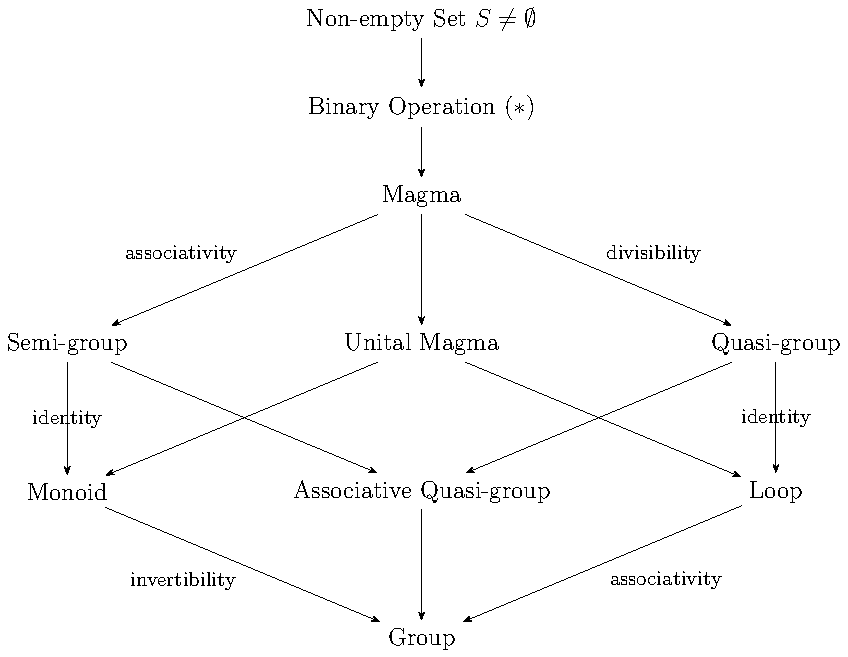
\includegraphics[width=\textwidth]{../tikz/grad-math-tikz-algebra/magamaTogroup.pdf}
\end{figure}
\vspace{20pt}
Algebraic structures are defined by sets equipped with one or more operations that satisfy specified axioms. These axioms guarantee, for example, that equations involving the operations behave in predictable ways. In this article we examine how the equation
\[
a\ast b = c
\]
(or its suitable variant) is interpreted in each context. We provide examples showing:
\begin{itemize}
	\item In a \emph{semigroup} the operation is associative and closed,
	\item In a \emph{monoid} an identity element exists,
	\item In a \emph{group} every element has an inverse (yielding unique solutions),
	\item In a \emph{module} equations can involve both the additive structure and scalar multiplication over a ring,
	\item In a \emph{vector space} (a module over a field) the additional invertibility of nonzero scalars facilitates solving linear equations.
\end{itemize}
\defbox[Binary Operation]{\begin{definition*}
Let \( S \) be a nonempty set. A \textbf{binary operation on} \( S \) is a function \[
* : S \times S \to S,
\] which assigns to each ordered pair $(a,b)\in S\times S$ an element $
*(a,b) = a*b\in S.$
\end{definition*}}
\begin{example}
A binary operation on a set $S$ is a rule that assigns to every ordered pair 
$(a,b)\in S$ an element $a*b\in S$. \begin{itemize}
	\item (Addition on Integers) Let $S=\Z$ and define \[
	+:\Z\times\Z\to\Z,\quad (a,b)\mapsto +(a,b)=a+b.
	\] This rule is a binary operation because the sum of any two integers is an integer.
	\item (Maximum of Two Real Numbers) Let $S=\R$ and define \[
	\fullfunction{\max}{\R\times\R}{\R}{(a,b)}{\max\set{a,b}}.
	\] For any two real numbers, their maximum is again a real number, so this is a valid binary operation.
\end{itemize}
\end{example}
\newpage
\defbox[Semi-group]{\begin{definition*}
A \textbf{semigroup} is an algebraic structure $(S,*)$ where:
\begin{enumerate}[(i)]
	\item $S\neq\varnothing$;
	\item $*:S\times S\to S$ is a binary operation that is \textit{associative} that is, for all $a,b,c\in S$, \[
	(a*b)*c\;=\; a*(b*c).
	\]
\end{enumerate}
\end{definition*}}

\begin{example}
A semigroup $(S,*)$ is a set $S$ together with a binary operation $*$ that is associative. \begin{itemize}
	\item (Positive Integers under Addition) Let $S=\Z^+=\set{1,2,3,\dots}$ and define addition as the operation. For $a,b,c\in\Z^+$, \[
	(a+b)+c=a+(b+c).
	\] and the sum of two positive integers is again a positive integer.
	\item (Singular Matrices under Multiplication) Let \[
	S:=\set{A\in M_{n\times n}(\R):\det(A)=0},\ \text{the set of all $n\times n$ singular matrices over $\R$},
	\] the set of all $n\times n$ singular matrices over $\R$, and define the operation as matrix multiplication.
	\begin{itemize}
		\item Associativity: Matrix multiplication is associative.
		\item Closure: If $A$ and $B$ are singular, then $\det(AB)=\det(A)\det(B)=0$; hence, $AB$ is singular.
	\end{itemize}
	Since the identity matrix (which is non-singular) is not in $S$, this semigroup does not have an identity element.
%	\item $(\set{0,1},\times)$ be a semigroup: \begin{table}[h!]\centering
%		\begin{tabular}{c||c|c}
%			& 0 & 1 \\ \hline\hline
%			0 & 0 & 0 \\ \hline
%			1 & 0 & 1 \\
%		\end{tabular}
%	\end{table}
\end{itemize}
\end{example}

\defbox[Monoid]{\begin{definition*}
A \textbf{monoid} is a semigroup \((S,\ast)\) that contains the \textit{identity element}. That is, there exists the element $e\in S$ such that for all $a\in S$. \[
e \ast a \;=\; a \;=\; a \ast e.
\]
\end{definition*}}
\begin{example}
A monoid is a semigroup that also has an identity element. \begin{itemize}
	\item (Nonnegative Integers under Addition) Let $S=\Z_{\geq 0}=\set{0,1,2,\dots}$ and define addition on $\Z_{\geq 0}$. \begin{itemize}
		\item Associativity: Addition is associative.
		\item Identity: The element $0\in\Z_{\geq 0}$ is the identity since \[
		0+a=a+0=a\quad \text{for each}\ a\in\Z_{\geq 0}.
		\]
	\end{itemize}
	\item (All Square Matrices under Multiplication) Let $S=M_n(\R)$, the set of all $n\times n$ matrices with real entries, and define the operation as matrix multiplication. \begin{itemize}
		\item Associativity: Matrix multiplication is associative.
		\item Identity: The identity matrix $I_n$ (with ones on the diagonal and zeros elsewhere) satisfies \[
		I_nA=A=AI_n\quad\text{for all}\ A\in M_n(\R).
		\]
	\end{itemize}
\end{itemize}
\end{example}


\defbox[Group]{\begin{definition*}
A \textbf{group} is a monoid \((S,\ast)\) in which every element has the \textit{inverse}. That is, for all $a\in S$, there exists the element $b\in S$ such that
\[
a \ast b \;=\; e \;=\; b\ast a.
\] Such \( b \in S \) is called an \emph{inverse} of \( a \), and is commonly denoted \( b=a^{-1} \).
\end{definition*}}
\begin{remark}
A \textbf{group} is an algebraic structure $(G,*)$ satisfying the following axioms:
\begin{enumerate}[(G1)]
	\item[\textcolor{gray}{(G0)}] \textcolor{gray}{(Closure) $\forall a,b\in G,\ a*b\in G$;}
	\item (Associativitiy) $\forall a,b,c\in G,\ (a*b)*c=a*(b*c)$;
	\item (Identity) $\exists e\in G:\forall a\in G,\ a*e=a=e*a$;
	\item (Inverse) $\forall a\in G,\ \exists\inv{a}\in G:\inv{a}*a=e=a*\inv{a}$.
\end{enumerate}
\end{remark}
\begin{example}
A group $(G,*)$ is a monoid in which every element has the inverse. \begin{itemize}
	\item (Integers under Addition) Let $G=\Z$ and define addition on $\Z$. \begin{itemize}
		\item Associativity: Addition is associative;
		\item Identity: The integer $0$ is the identity;
		\item Inverse: For every $a\in\Z$, the element $-a\in\Z$ is its inverse since $a+(-a)=0=(-a)+a$. 
	\end{itemize}
	This group is abelian because addition is commutative.
	\item (General Linear Group) Let \[
	G=GL(n,\R)=\set{A\in M_n(\R):\det(A)\neq 0},
	\] with the operation of matrix multiplication. \begin{itemize}
		\item Associativity: Matrix multiplication is associative.
		\item Identity: The identity matrix $I_n$ is the identity.
		\item Inverse: Every matrix in $GL(n,\R)$ is invertible. This group is generally non-abelian.
	\end{itemize}
\end{itemize}
\end{example}


\begin{remark}
Let \(G\) be a set equipped with a binary operation \(*\). In particular, if
\[
\forall\, a,b\in G,\quad a * b = b * a,
\]
then the group \(G\) is said to be \textbf{commutative} (or \textbf{abelian}). That is, an algebraic structure $(G,*)$ is an abelian group if and only if:
\begin{enumerate}[(G1)]
	\item[\textbf{(G0)}] \textbf{Closure:} $
	\forall\, a,b\in G:\quad a+b\in G.$
	\item[\textbf{(G1)}] \textbf{Associativity:} \(\forall a,b,c\in G\), $
	(a+b)+c = a+(b+c).$
	\item[\textbf{(G2)}] \textbf{Identity:} \(\exists 0\in G\) such that \(\forall a\in G\),\ $a+0 = a = 0+a.$
	\item[\textbf{(G3)}] $\forall a\in G$,\ $\exists -a\in G$ such that
	$(-a)+a = 0 = a+(-a).$
	\item[\textbf{(C)}] \textbf{Commutativity:} \(\forall a,b\in G\),\ $
	a+b = b+a.$
\end{enumerate}
\end{remark}
\begin{example}
\ \begin{itemize}
	\item $(\N,+)$ is a semigroup but is not monoid.
	\item $(\N,\times)$ is a monoid but is not group.
	\item $(\Z,+)$ is a group.
	\item $(\Q,+)$ is a group.
	\item $(\R,+)$ is a group.
	\item $(\Z\setminus\set{0},\times)$ is a semigroup.
	\item $(\Q\setminus\set{0},\times)$ is a group.
	\item $(\R\setminus\set{0},\times)$ is a group.
	\item $(GL_n(\R),*)$ is a group, where \[
	GL_n(\R):=\set{A\in M_n(\R):\det A\neq 0}
	\] and $*$ is the matrix multiplication.
	\item $(\mathcal{F},\circ)$ is a group, where \[
	\mathcal{F}:=\set{f\in A^A:\ \text{$f$ is one-to-one and onto}}
	\] and $\circ$ is the composition of functions.
\end{itemize}
\end{example}
\begin{example}[Lie-bracket]
	content...
\end{example}

\probox{\begin{proposition}
Let $G$ be a group with $*$ (normally omitted). Then \begin{enumerate}[(1)]
	\item $\exists! e\in G$;
	\item $\exists!\inv{a}$
	\item $\forall a\in G:\inv{\of{\inv{a}}}=a$
	\item $\forall a,b\in G:\inv{ab}=\inv{b}\inv{a}$
	\item (Generalized Associative Law) for any $a_1,a_2,\dots, a_n\in G$, the value of $a_1*a_2*\cdots*a_n$ is independent of how the expression is bracketed.
\end{enumerate}
\end{proposition}}
\begin{proof}
	content...
\end{proof}

\defbox[Ring]{\begin{definition*}
A \textbf{ring} is an algebraic structure $(R,+,\cdot)$ where: \begin{enumerate}[(i)]
	\item $(R,+)$ is an abelian group with identity element $0$: that is, for all $a,b,c\in R$: \begin{itemize}
		\item Associativity: $(a+b)+c=a+(b+c)$;
		\item Commutativity: $a+b=b+a$;
		\item Identity: There exists $0\in R$ such that $a+0=a$;
		\item Inverse: For every $a\in R$, there exits an element $-a\in R$ with $a+(-a)=0$.
	\end{itemize}
	\item $(R,\cdot)$ is a semigroup; that is, multiplication is \textit{associative}: \[
	(a\cdot b)\cdot c=a\cdot (b\cdot c)\quad\text{for all}\ a,b,c\in R.
	\]
	\item Distributivity: Multiplication is distributive over addition: \begin{align*}
		a\cdot (b+c)&=a\cdot b+a\cdot c\quad\text{and} \\
		(a+b)\cdot c&=a\cdot c+b\cdot c
	\end{align*} for all $a,b,c\in R$.
\end{enumerate}
\end{definition*}\tcblower
\color{gray!50} Some authors require the existence of a multiplicative identity (an element $1\in R$ such that $1\cdot a=a=a\cdot 1$ for all $a\in R$); if so, the ring is called a ring with unity.}
\begin{example}
\ \begin{itemize}
	\item (The Integers $\Z$) Consider $R=\Z$ with the usual addition and multiplication.
	\begin{itemize}
		\item $(\Z,+)$ is an abelian group (with identity $0$).
		\item Multiplication is associative.
		\item The distributive laws hold, \ie, $a(b+c)=ab+ac$ and $(a+b)c=ac+bc$ for all $a,b,c\in\Z$.
	\end{itemize}
	This ring is also commutative and has a multiplicative identity $1$.
	\item (Polynomial Ring $\C[x]$) Let $R=\C[x]$, the set of all polynomials in $x$ with complex coefficients. \begin{itemize}
		\item $(\C[x],+)$ is an abelian group (with the zero polynomial $0$ as the identity).
		\item Polynomial multiplication is associative.
		\item The distributive laws hold, \ie, $f(x)(g(x)+h(x))=f(x)g(x)+f(x)h(x)$ and $(f(x)+g(x))h(x)=f(x)h(x)+g(x)h(x)$ for all $f(x),g(x),h(x)\in\C[x]$.
	\end{itemize}
	This ring is also commutative and has a multiplicative identity $1$ (the constant polynomial $1$).
\end{itemize}
\end{example}

\defbox[Field]{\begin{definition*}
A \textbf{field} an algebraic structure $(F,+,\cdot)$ such that \begin{enumerate}[(i)]
	\item $(F,+)$ is an abelian group with additive identity element $0$;
	\item $(F\setminus\set{0},\cdot)$ is an abelian group with multiplicative identity element $1$, where $0\neq 1$;
	\item Distributivity: Multiplication is distributive over addition; that is, for all $a,b,c\in F$, \[
	a\cdot (b+c)=a\cdot b+a\cdot c.
	\]
\end{enumerate} 
\end{definition*}}
\begin{example}
A field is a commutative ring with unity in which every nonzero element is invertible under multiplication. \begin{itemize}
	\item (The Real Numbers $\R$) Let $F=\R$ with the usual addition and multiplication. \begin{itemize}
		\item $(\R,+)$ is an abelian group (with $0$ as the additive identity)
		\item $(\R\setminus\set{0},\cdot)$ is an abelian group (with $1$ as the multiplicative identity)
		\item Multiplicative distributes over addition.
	\end{itemize}
	\item (Finite Field $\Z_p$) Let $p$ be a prime number and define \[
	\Z_p:=\set{0,1,\dots, p-1},
	\] with addition and multiplication defined modulo $p$. \begin{itemize}
		\item $(\Z_p,+)$ is an abelian group with the additive identity $0$.
		\item $(\Z_p\setminus\set{0},\cdot)$ is an abelian group with the multiplicative identity $1$ since every nonzero element has a unique inverse module $p$\footnote{By Bézout's identity, for $a,b\in\Z$, $\exists x,y\in\Z$ s.t. $ax+by=\gcd(a,b)$. Let $p$ be a prime. Then for any integer $a\in\Z$, $\exists x,y$ s.t. $ax+py=\gcd(a,p)=1$, and so $ax\equiv 1\pmod{p}$.}.
		\item The distributive laws hold modulo $p$.
	\end{itemize}
\end{itemize}
\end{example}

\defbox[Module]{\begin{definition*}
Let \( R \) be a ring with unity $1_R$. An $R$-\textbf{module} is an structure $(M,+,\cdot)$ consisting of an abelian group $(M,+)$ together with a scalar multiplication \[
\cdot:R\times M\to M
\] that satisfies the following axioms for all $r,s\in R$ and $m,n\in M$:
\begin{enumerate}[(i)]
	\item Distributivity over Module Addition: \[
	r \cdot (m+n) = r \cdot m + r \cdot n,
	\]
	\item Distributivity over Ring Addition: \[
	(r+s) \cdot m = r \cdot m + s \cdot m,
	\]
	\item Associativity of Scalar Multiplication: \[
	(rs) \cdot m = r \cdot (s \cdot m),
	\]
	\item Unital Property (if $R$ is unital): \[
	1_R \cdot m = m.
	\]
\end{enumerate}
\end{definition*}}


\defbox[Vector Space]{\begin{definition*}
Let \( F \) be a field. A \emph{vector space} over \( F \) is a structure \((V, +, \cdot)\) satisfying:
\begin{enumerate}[(i)]
	\item \( V \neq \varnothing \).
	\item \((V, +)\) is an abelian group with identity element \( 0 \in V \).
	\item \(\cdot : F \times V \to V\) is a function called \emph{scalar multiplication}.
	\item The following axioms hold:
	\[
	\forall\, a,b \in F,\ \forall\, u,v \in V: \quad a \cdot (u+v) = a \cdot u + a \cdot v,
	\]
	\[
	\forall\, a,b \in F,\ \forall\, v \in V: \quad (a+b) \cdot v = a \cdot v + b \cdot v,
	\]
	\[
	\forall\, a,b \in F,\ \forall\, v \in V: \quad a \cdot (b \cdot v) = (a b) \cdot v,
	\]
	\[
	\forall\, v \in V: \quad 1_F \cdot v = v,
	\]
	where \(1_F\) denotes the multiplicative identity in \( F \).
\end{enumerate} This is, given a field $F$, we say $V$ is a vector space over $F$ if $V$ is a $F$-module
%Thus, formally,
%\[
%(V, +, \cdot) \text{ is a vector space over } F \iff
%\]
%\[
%\left[
%\begin{array}{l}
%	V \neq \varnothing, \\
%	(V, +) \text{ is an abelian group with identity } 0, \\
%	\cdot : F \times V \to V, \\
%	\forall\, a,b\in F,\ \forall\, u,v\in V:\quad a \cdot (u+v) = a \cdot u + a \cdot v,\\[1mm]
%	\forall\, a,b\in F,\ \forall\, v\in V:\quad (a+b) \cdot v = a \cdot v + b \cdot v,\\[1mm]
%	\forall\, a,b\in F,\ \forall\, v\in V:\quad a \cdot (b \cdot v) = (ab) \cdot v,\\[1mm]
%	\forall\, v\in V:\quad 1_F \cdot v = v.
%\end{array}
%\right]
%\]		
\end{definition*}}

\defbox[Algebra]{\begin{definition*}
	Given a ring $R$ and a set $A$, we say $A$ is the algebra if $A$ has three operators: with compatabilitiy
\end{definition*}}

\newpage

\section{Introduction}


\section{Semigroups}
\begin{definition}[Semigroup]
	A \emph{semigroup} is a pair \((S,\ast)\) where \(S\) is a nonempty set and
	\[
	\ast: S \times S \to S
	\]
	is a binary operation satisfying the associativity axiom:
	\[
	\forall\, a,b,c \in S,\quad (a\ast b)\ast c = a\ast (b\ast c).
	\]
\end{definition}

In a semigroup the equation
\[
a\ast b = c
\]
illustrates that the result is always an element of \(S\) (closure), and the grouping of operations is unambiguous (associativity). However, since there is no guarantee of an identity or inverses, solving for one variable given the others may not be possible or unique.

\subsection*{Example 1 (Addition on \(\mathbb{N}\))} 
Let \(S=\mathbb{N}=\{1,2,3,\dots\}\) and define \(\ast\) as addition. Then:
\[
3+ b = 7 \quad \Longrightarrow \quad b=4,
\]
provided that \(7\ge 3\). Note that if we choose \(a=5\) and \(c=3\), no solution exists in \(\mathbb{N}\).

\subsection*{Example 2 (String Concatenation)}
Let \(S\) be the set of all nonempty strings over a fixed alphabet and define \(\ast\) as concatenation. For instance, with
\[
a = \text{``Hello''}, \quad b = \text{``World''},
\]
we have
\[
a \ast b = \text{``HelloWorld''}.
\]
In this semigroup, while concatenation is associative and closed, an equation like
\[
a \ast x = c,
\]
may have multiple or no solutions because the decomposition of \(c\) is not necessarily unique.

\section{Monoids}
\begin{definition}[Monoid]
	A \emph{monoid} is a semigroup \((M,\ast)\) that contains an \emph{identity element} \(e\) satisfying:
	\[
	\forall\, a \in M,\quad a\ast e = e\ast a = a.
	\]
\end{definition}

In a monoid the equation
\[
a\ast b = c
\]
may be interpreted using the identity. However, without the existence of inverses, “solving” such equations (i.e., undoing the operation) is not always possible.

\subsection*{Example 1 (Nonnegative Integers \(\mathbb{N}_0\) Under Addition)}
Let \(M=\mathbb{N}_0 = \{0,1,2,\dots\}\) with addition and \(0\) as the identity. Then:
\[
3+b=7 \quad \Longrightarrow \quad b=4.
\]
Conversely, if \(a=8\) and \(c=5\), there is no \(b\in \mathbb{N}_0\) satisfying
\[
8+b=5,
\]
since subtraction may lead out of \(\mathbb{N}_0\).

\subsection*{Example 2 (Strings Including the Empty String)}
Let \(M\) be the set of all finite strings over an alphabet including the empty string \(\varepsilon\), with concatenation as the operation. The empty string acts as the identity:
\[
\varepsilon \ast s = s \ast \varepsilon = s.
\]
For the equation
\[
\text{``Hi''} \ast x = \text{``HiThere''},
\]
one solution is
\[
x = \text{``There''}.
\]
Again, note that the lack of invertibility means that not every such equation is guaranteed to have a solution.

\section{Groups}
\begin{definition}[Group]
	A \emph{group} is a monoid \((G,\ast)\) in which every element has an inverse. That is,
	\[
	\forall\, a \in G,\quad \exists\, a^{-1} \in G \text{ such that } a\ast a^{-1} = a^{-1}\ast a = e.
	\]
\end{definition}

In a group the equation
\[
a\ast b = c
\]
has the additional property that a unique solution exists for any one of the variables. This is because the existence of inverses allows us to “undo” the operation.

\subsection*{Example 1 (Integers Under Addition)}
Let \(G=\mathbb{Z}\) with addition. Given
\[
a+b = c,
\]
for any \(a,c\in \mathbb{Z}\) the unique solution for \(b\) is
\[
b=c-a.
\]
For example, if \(3+b=7\), then \(b=7-3=4\).

\subsection*{Example 2 (Nonzero Real Numbers Under Multiplication)}
Consider the group \(G=\mathbb{R}^*=\mathbb{R}\setminus\{0\}\) with multiplication. The equation
\[
a\cdot b = c,
\]
has the unique solution
\[
b = \frac{c}{a},
\]
since every nonzero real number \(a\) has an inverse \(a^{-1}=\frac{1}{a}\). For instance, if \(2\cdot b=8\), then \(b=\frac{8}{2}=4\).

\section{Modules}
\begin{definition}[Module]
	Let \(R\) be a ring with unity. A \emph{module} over \(R\) is a triple \((M, +, \cdot)\) where:
	\begin{enumerate}[(i)]
		\item \((M,+)\) is an abelian group (with identity \(0\)),
		\item \(\cdot : R \times M \to M\) is scalar multiplication,
		\item The following axioms hold for all \(r,s \in R\) and \(m,n \in M\):
		\[
		r\cdot(m+n)=r\cdot m + r\cdot n,
		\]
		\[
		(r+s)\cdot m = r\cdot m + s\cdot m,
		\]
		\[
		(rs)\cdot m = r\cdot(s\cdot m),
		\]
		\[
		1_R\cdot m = m.
		\]
	\end{enumerate}
\end{definition}

In a module, equations may involve both the additive structure and scalar multiplication. For example, the equation
\[
r\cdot x = m
\]
asks for an element \(x\in M\) such that when scaled by \(r\in R\) the result is \(m\).

\subsection*{Example 1 (The \(\mathbb{Z}\)-Module \(\mathbb{Z}\))}
View \(\mathbb{Z}\) as a module over itself. Consider:
\[
2\cdot x = 6.
\]
Since scalar multiplication in a \(\mathbb{Z}\)-module is just ordinary multiplication, the solution is \(x=3\). In contrast, the equation
\[
2\cdot x = 5
\]
has no solution in \(\mathbb{Z}\) because \(5\) is not an even number.

\subsection*{Example 2 (A Linear Equation in \(\mathbb{Z}^2\))}
Let \(M=\mathbb{Z}^2\) be a \(\mathbb{Z}\)-module and consider the equation
\[
2\cdot (x_1,x_2) + 3\cdot (y_1,y_2) = (8,11).
\]
This expands to the system of linear Diophantine equations:
\[
2x_1+3y_1 = 8, \quad 2x_2+3y_2 = 11.
\]
Solutions exist if and only if each coordinate equation is consistent in \(\mathbb{Z}\).

\section{Vector Spaces}
\begin{definition}[Vector Space]
	Let \(F\) be a field. A \emph{vector space} over \(F\) is a module \((V,+,\cdot)\) satisfying the module axioms (with \(F\) replacing \(R\)) and, importantly, where every nonzero scalar in \(F\) is invertible.
\end{definition}

Equations in a vector space benefit from both the additive structure and the rich scalar multiplication properties provided by the field.

\subsection*{Example 1 (Vector Addition in \(\mathbb{R}^2\))}
Let \(V=\mathbb{R}^2\). Consider the equation
\[
v + w = z.
\]
If
\[
v = (1,2) \quad \text{and} \quad z = (4,7),
\]
then solving for \(w\) gives
\[
w = z - v = (4-1,7-2) = (3,5).
\]

\subsection*{Example 2 (Scalar Multiplication in \(\mathbb{R}^2\))}
In the vector space \(V=\mathbb{R}^2\), consider the equation
\[
c \cdot v = w,
\]
with \(v=(2,3)\) and \(w=(4,6)\). Since scalar multiplication is defined coordinate-wise and \(c\) is a scalar from \(\mathbb{R}\), we obtain
\[
c = \frac{4}{2} = 2,
\]
which is unique because nonzero scalars in a field are invertible.

\section{Conclusion}
The equation \(a\ast b = c\) (or its variants) encapsulates different aspects of algebraic structures:
\begin{itemize}
	\item In a \textbf{semigroup}, closure and associativity guarantee that the operation is well-defined.
	\item In a \textbf{monoid}, the presence of an identity element allows for the natural “do-nothing” solution.
	\item In a \textbf{group}, every equation has a unique solution thanks to the existence of inverses.
	\item In a \textbf{module} and a \textbf{vector space}, additional structure from scalar multiplication enables the formulation and solution of linear equations.
\end{itemize}
These examples highlight how the abstract axioms influence the process of solving equations in each setting, providing a concrete interpretation of the algebraic structures.

\newpage

\section{Semigroups}
\begin{definition}[Semigroup]
	A \emph{semigroup} is a set \(S\) together with a binary operation 
	\[
	\ast: S\times S \to S,
	\]
	which is associative:
	\[
	\forall\, a,b,c\in S,\quad (a\ast b)\ast c = a\ast (b\ast c).
	\]
\end{definition}

In a semigroup, the equation
\[
a\ast b = c
\]
always yields an element \(c\in S\) (closure), and the grouping of operations is unambiguous (associativity). However, there is no requirement for an identity or inverses, so solving such equations (i.e., “undoing” the operation) may not be feasible or unique.

\begin{example}[Non-empty Strings under Concatenation]
	Let \(S\) be the set of all non-empty finite strings over a fixed alphabet (e.g., \(\{a,b,c,\dots\}\)), and define the operation \(\ast\) as concatenation. For any strings \(s,t\in S\), the concatenation \(s\ast t\) is again a non-empty string, and concatenation is associative:
	\[
	(s\ast t)\ast u = s\ast (t\ast u).
	\]
	Since the empty string is excluded, there is no identity element. Thus, \((S,\ast)\) is a semigroup.
\end{example}

\begin{example}[Positive Integers (Excluding 1) under Multiplication]
	Define 
	\[
	S = \{n\in \mathbb{N} : n \ge 2\},
	\]
	and let the operation \(\ast\) be ordinary multiplication. Since
	\[
	a\ast b = ab \in S \quad \text{for all } a,b \ge 2,
	\]
	and multiplication is associative, \((S, \times)\) is a semigroup. Note that the multiplicative identity \(1\) is not in \(S\), so no identity element exists.
\end{example}

\section{Monoids}
\begin{definition}[Monoid]
	A \emph{monoid} is a semigroup \((M, \ast)\) that contains an identity element \(e\) such that
	\[
	\forall\, a \in M,\quad e\ast a = a\ast e = a.
	\]
\end{definition}

In a monoid the equation
\[
a\ast b = c
\]
can sometimes be “undone” by using the identity element—but without inverses, one cannot generally solve for an unknown.

\begin{example}[Natural Numbers with Zero under Addition]
	Let
	\[
	M = \mathbb{N}_0 = \{0,1,2,\dots\},
	\]
	with the operation \(+\). Since addition is associative, and \(0\) serves as the identity element (because \(0+a=a+0=a\)), \((\mathbb{N}_0, +)\) is a monoid. Notice that aside from \(0\), no element has an additive inverse in \(\mathbb{N}_0\).
\end{example}

\begin{example}[All Finite Strings (Including the Empty String) under Concatenation]
	Let \(M\) be the set of all finite strings over a fixed alphabet, \emph{including} the empty string \(\varepsilon\). Define the operation as concatenation. The empty string \(\varepsilon\) acts as the identity since
	\[
	\varepsilon \ast s = s \ast \varepsilon = s,
	\]
	for every string \(s\). Thus, \((M,\ast)\) is a monoid. This example is non-trivial because the set \(M\) is infinite and diverse in structure.
\end{example}

\section{Groups}
\begin{definition}[Group]
	A \emph{group} is a monoid \((G, \ast)\) in which every element has an inverse. That is,
	\[
	\forall\, a \in G,\quad \exists\, a^{-1} \in G \text{ such that } a\ast a^{-1} = a^{-1}\ast a = e.
	\]
\end{definition}

In a group every equation of the form
\[
a\ast b = c
\]
can be uniquely solved for any one variable by “canceling” with the inverse.

\begin{example}[Integers under Addition]
	Let
	\[
	G = \mathbb{Z},
	\]
	with the operation \(+\). The identity element is \(0\) (since \(a+0=0+a=a\) for all \(a\in\mathbb{Z}\)), and every integer \(a\) has the inverse \(-a\) (because \(a+(-a)=0\)). Hence, \((\mathbb{Z},+)\) is a group. For example, the equation
	\[
	3 + b = 7
	\]
	has the unique solution \(b=7-3=4\).
\end{example}

\begin{example}[The Symmetric Group \(S_3\)]
	The symmetric group \(S_3\) is the set of all permutations of three objects, with the operation being composition of functions. The identity permutation (which leaves all elements fixed) serves as the identity element. Every permutation in \(S_3\) has an inverse (its inverse permutation), and composition is associative. Since \(S_3\) is non-abelian (the order of composition matters), it provides a non-trivial example of a finite group.
\end{example}

\section{Modules}
\begin{definition}[Module]
	Let \(R\) be a ring with unity. An \emph{\(R\)-module} \(M\) is an abelian group \((M, +)\) equipped with a scalar multiplication
	\[
	\cdot: R \times M \to M,
	\]
	satisfying, for all \(r,s\in R\) and \(m,n\in M\):
	\[
	r\cdot (m+n)=r\cdot m + r\cdot n, \quad (r+s)\cdot m = r\cdot m + s\cdot m,
	\]
	\[
	(rs)\cdot m = r\cdot (s\cdot m), \quad 1_R\cdot m = m.
	\]
\end{definition}

In modules, equations may involve both the additive structure and the action of scalars from the ring \(R\).

\begin{example}[\(\mathbb{Z}^2\) as a \(\mathbb{Z}\)-Module]
	Let
	\[
	M=\mathbb{Z}^2 = \{ (a,b) \mid a,b\in \mathbb{Z} \},
	\]
	with vector addition defined componentwise and scalar multiplication by an integer \(k\) given by
	\[
	k\cdot (a,b) = (ka, kb).
	\]
	Since \(\mathbb{Z}^2\) is an abelian group under addition and the scalar multiplication satisfies the module axioms over the ring \(\mathbb{Z}\), it forms a non-trivial \(\mathbb{Z}\)-module.
\end{example}

\begin{example}[\(\mathbb{Z}_6\) as a \(\mathbb{Z}\)-Module]
	Let
	\[
	M=\mathbb{Z}_6 = \{\, [0], [1], [2], [3], [4], [5] \,\},
	\]
	the integers modulo 6, with addition modulo 6. Every abelian group is naturally a \(\mathbb{Z}\)-module via the operation
	\[
	k\cdot [a] = [ka],
	\]
	with the usual multiplication of integers followed by reduction modulo 6. Thus, \(\mathbb{Z}_6\) is a non-trivial, finite \(\mathbb{Z}\)-module.
\end{example}

\section{Vector Spaces}
\begin{definition}[Vector Space]
	Let \(F\) be a field. A \emph{vector space} \(V\) over \(F\) is an \(F\)-module (i.e., an abelian group \((V, +)\) with a scalar multiplication \(\cdot: F\times V \to V\)) satisfying all the module axioms, where every nonzero scalar has a multiplicative inverse.
\end{definition}

In vector spaces the availability of multiplicative inverses for scalars (when nonzero) ensures that linear equations have unique solutions.

\begin{example}[\(\mathbb{R}^3\)]
	Let
	\[
	V = \mathbb{R}^3 = \{ (x,y,z) \mid x,y,z\in\mathbb{R} \},
	\]
	with the usual vector addition and scalar multiplication. This three-dimensional vector space over \(\mathbb{R}\) is a classic example where the equation
	\[
	v + w = u
	\]
	has a unique solution for any one of the vectors when the other two are known.
\end{example}

\begin{example}[The Space of Polynomials \(P_2(\mathbb{R})\)]
	Let
	\[
	V = P_2(\mathbb{R}) = \{\, a_0 + a_1 x + a_2 x^2 \mid a_0,a_1,a_2 \in \mathbb{R} \,\},
	\]
	the set of all real polynomials of degree at most 2. With polynomial addition and scalar multiplication defined in the usual way, \(P_2(\mathbb{R})\) forms a vector space over \(\mathbb{R}\). This space is non-trivial and is widely used in approximation theory and other applications.
\end{example}

\section{Conclusion}
We have presented two non-trivial, concrete examples for each of the algebraic structures considered:
\begin{itemize}
	\item \textbf{Semigroups:} non-empty strings under concatenation and positive integers (excluding 1) under multiplication.
	\item \textbf{Monoids:} natural numbers (including zero) under addition and all finite strings (including the empty string) under concatenation.
	\item \textbf{Groups:} the group of integers under addition and the symmetric group \(S_3\).
	\item \textbf{Modules:} \(\mathbb{Z}^2\) and \(\mathbb{Z}_6\) as \(\mathbb{Z}\)-modules.
	\item \textbf{Vector Spaces:} the three-dimensional real space \(\mathbb{R}^3\) and the space of polynomials \(P_2(\mathbb{R})\).
\end{itemize}
In each case, the underlying operation ensures that equations such as \(a\ast b = c\) are well defined, and the additional axioms (e.g., existence of an identity or inverses) dictate the nature of solution methods within that structure.


\begin{thebibliography}{9}
	\bibitem{algebra_0}
	수학의 즐거움, Enjoying Math. ``수학 공부, 기초부터 대학원 수학까지, 13. 대수학 : 군, 환, 체, 가군, 벡터공간, 대수의 정의'' YouTube Video, 25:57. Published 
	October 7, 2019. URL: \url{https://www.youtube.com/watch?v=6DP6UQ2sPus}.
\end{thebibliography}

\end{document}
